\pagestyle{fancy}
\fancyhf{}
\renewcommand{\headrulewidth}{0pt}
\fancyfoot[C]{\leftmark}
\fancyhead[R]{\thepage}
\doublespacing
\chapter{Poiseuille flow of soft glass: role of thermalization protocol}\label{chap5}

\noindent\fbox{\parbox{\textwidth}
    {\color{myred}
    This chapter is based on the following publication \cite{vaibhav2021influence}:\\
    {\em Influence of thermalisation protocol on Poiseuille flow of confined soft glass}\\
    V. Vaibhav, and P. Chaudhuri, Physics of Fluids 33, 053103 (2021)}
}


\section{Introduction}

Soft glassy materials are all around us, both in nature and daily lives. In general, all glassy systems are characterised by the existence of a yield stress \cite{coussot2014yield, bonn2017yield, joshi2018yield}, i.e. a finite stress threshold needs to be overcome in order for the material to yield. For soft glasses (e.g. colloids, emulsions, gels, granular suspensions etc.), steady flow is observed once this yield threshold has been crossed, and this property has been utilised in diverse important applications. Prior to the onset of steady flow, fascinating spatio-temporal behaviour \cite{rodney2011modeling} is observed which are linked to the  occurrence of spatially correlated plastic events \cite{bocquet2009kinetic, nicolas2018deformation}, the cascade of which leads to yielding and flow. Such correlated processes continue in steady state and the bulk rheological flow curves are well described by the Herschel Bulkley function \cite{bonn2017yield}. Overall,
understanding and characterising the diverse rheological response \cite{bonn2017yield, joshi2018yield, tanner2018aspects, semwogerere2008shear, khabaz2021thermodynamics, jacob2019rheological, agarwal2019signatures, biswas2021quantifying, sriram2010active} of soft glassy materials has been actively undertaken to help in improving existing applications or design new materials with specific functions.

One of the possible ways to study the rheological response of soft glassy systems is via Poiseuille flow (check section-\ref{PoiseuilleFlow} of Chapter-\ref{chap1} for basic introduction to Poiseuille flow), which has become quite significant in the context of microfluidic devices \cite{tabeling2005introduction}, 3d printing \cite{zhu2019colloidal, nelson2020embedded} and also applications involving extrusion of materials \cite{ebendorff2007extrusion}, and therefore has been investigated via experiments \cite{goyon2008spatial, isa2009velocity, genovese2011crystallization, ballesta2012wall, nordstrom2010microfluidic}, numerical simulations \cite{chaudhuri2012dynamical, mansard2013molecular, pinaki2014, lulli2018metastability} and different coarse-grained models \cite{nicolas2013mesoscopic, papenkort2014channel, lulli2018metastability}. In the case of Poiseuille flow, the pressure gradient applied across the channel leads to the occurrence of a spatially non-uniform stress field across the width of the channel in the flow gradient plane. In the presence of an inhomogeneous stress field, the naive expectation is that  the material will flow, i.e. there will be finite shear-rate, wherever the local stress is above the yield stress. For Poiseuille flow, this would lead to blunted velocity profiles for soft glasses \cite{PhysRevE.77.011504} instead of the parabolic velocity profiles that occur for Newtonian fluids \cite{evansMorrissBook}. However, it was demonstrated that due to the interplay between the spatially correlated plasticity occurring in glassy systems, as discussed above, and the stress gradients that are characteristic to Poiseuille flow, there not only exists a macroscopic yield threshold that depends upon the channel width \cite{chaudhuri2012dynamical} but also the observed velocity profiles  deviate from those predicted from the Herschel-Bulkley bulk rheology, with the deviation increasing with decreasing channel width \cite{goyon2008spatial, mansard2013molecular}. Due to this fascinating non-local coupling, the onset of flow also takes place collectively across the channel, and hysteresis linked to metastable states are also observed in thermal systems \cite{pinaki2014, lulli2018metastability}.  Further, it has been demonstrated that due to such spatial correlations occurring during the flow, the rheological behaviour can be greatly influenced by the roughness of the confining walls of the channel \cite{mansard2014boundary}, which thus provides a design control for various applications. 


\section{Objective}

%In this work, we investigate a similar boundary driven effect, albeit in a different way. 
Previous studies \cite{baranyai1992isothermal} have demonstrated that in the presence of a spatially varying shear-rate, heat flow can occur even in the absence of any externally applied thermal gradient. Further, it was illustrated that for the case of Poiseuile flow of a fluid confined between walls via which temperature control is maintained, a spatially varying temperature profile emerges in steady state, which has a quartic spatial dependence as predicted from solutions of phenomenological hydrodynamic equations \cite{todd1995, varnik2002, binder2004molecular}. Motivated by this phenomenon, we investigate how such thermalised boundaries influence the Poiseuille flow of a model soft glass, both in steady state and also during the onset of flow from a quiescent state. We contrast our observations with the case where the confined fluid is thermalised directly, and not via the walls. Our main objective is to study the rheological response of a soft glass in the simultaneous presence of a local stress gradient (via the Poiseuille setup) and a local temperature gradient (via the temperature control using walls), and contrast that with the situation where the thermal gradient is absent during the Poiseuille flow. Thus, it is not a study of the efficacy of the two different kinds of thermostats, but rather investigating the rheological consequence of having non-uniform temperature within the channel during the Poiseuille flow. In the broader context, such a study is part of recent investigations into the role of dissipation processes \cite{nicolas2016effects, irani2019discontinuous, vasisht2018permanent} in determining the non-equilibrium response of sheared amorphous materials. 

%The paper is organised as follows. After the introductory note in Section I, in Section II, we discuss the model glass former that is studied, the method for setting up the Poiseuille flow for the glass confined between rough walls, and the methods for the two studied thermostats, viz. in one case, where the confined fluid is thermalised via the walls and another case, where the fluid is directly thermalised. In Section III, we discuss the results of our study, probing the behaviour in the quiescent state, and in the driven state, both in steady state as well as during the onset of flow. Further, we also discuss, in the same section, a brief comparison of response across varying channel widths. Finally, in section IV, we provide some concluding discussions.

                                                        
\section{Model and methods}

\subsection{The model glass former}

In this work, we consider the well-studied glass-forming model binary Lennard-Jones mixture \cite{Kob94} (check section-\ref{model} of Chapter-\ref{chap2} for more details about the model), whose rheological properties have been well characterized in terms of well-known soft glass phenomenology. 

All lengths are measured in the unit of $\sigma_{\rm AA}$, energy is expressed in the units of $\varepsilon_{\rm AA}$, the unit of time is $\sqrt{{m\sigma_{\rm AA}^{2}}/\epsilon_{\rm AA}}$ and that of stress is $\epsilon_{\rm AA}/ \sigma_{\rm AA}^{3}$. For this mixture,  the increase in relaxation timescales of the supercooled liquid with decreasing temperature can be fitted with mode coupling theory prediction, providing a mode-coupling critical temperature $T_{MCT} \approx 0.435$, below which conventional numerical simulations fail to obtain equilibrium dynamics. However, the putative glass transition temperature of the system, $T_{VFT} \approx 0.3$ is obtained by a Vogel-Fulcher-Tammam fit to the variation of relaxation timescale with temperature. We study the flow response of the mixture at $T_0=0.40$, which is in between  $T_{MCT}$ and $T_{VFT}$, i.e. within the thermal aging regime. We carry out extensive molecular dynamics simulations to study the response to external shear using  LAMMPS \cite{lammps}, with the equations of motion being integrated via velocity-Verlet scheme with time-step $\Delta t = 0.005$.

\subsection{Poiseuille flow}

For the purpose of studying channel flow, we initially consider a periodic rectangular box of dimension $L_x \times L_y \times L_z$, extended between $0$ to $L_x$ along $x$, $0$ to $L_y$ along $y$ and  $-L_z/2$ to $L_z/2$  along $z$. Different independent initial states are prepared by quenching well-equilibrated high temperature configurations at $T=5.0$  to $T=0.4$ below $T_{MCT}$, which are subsequently aged for a duration of $t_{age} = 10^4$. The particles in the two regions parallel to $xy$ plane for which $|z| > L_z/2 -3$ make the two amorphous walls (each of thickness $3 \sigma_{\rm AA}$) which confine the system to make a channel of width $L_z-6$. This construction of the walls is done after the aging process has been completed following the quench from $T=5.0$  to $T=0.4$. To implement Poiseuille flow, a force $F_x$ is applied on all the particles in the confined channel along $x$-direction \cite{todd1995pressure}. 


In this work, we study the Poisueille flow in channels of two different widths, viz. $w=100, 25$. For that purpose, we use two different sample sizes having roughly same number of fluid particles: $30 \times 30 \times 106$ (114 480 particles) and $120 \times 30 \times 31$ (133 920 particles), taking into account the confinement via walls. Most of the results are reported for channel $w=100$ and at the end, we provide a brief comparison with observations in $w=25$. The choice of the wider channel for the present study is led by the focus on investigating the role of thermal gradients in rheology, with smaller interference from effects due to confinement, which we will also briefly probe as indicated. All reported results are averaged over 10-30 independent trajectories.


%%%%%%%
\begin{figure}
\centering
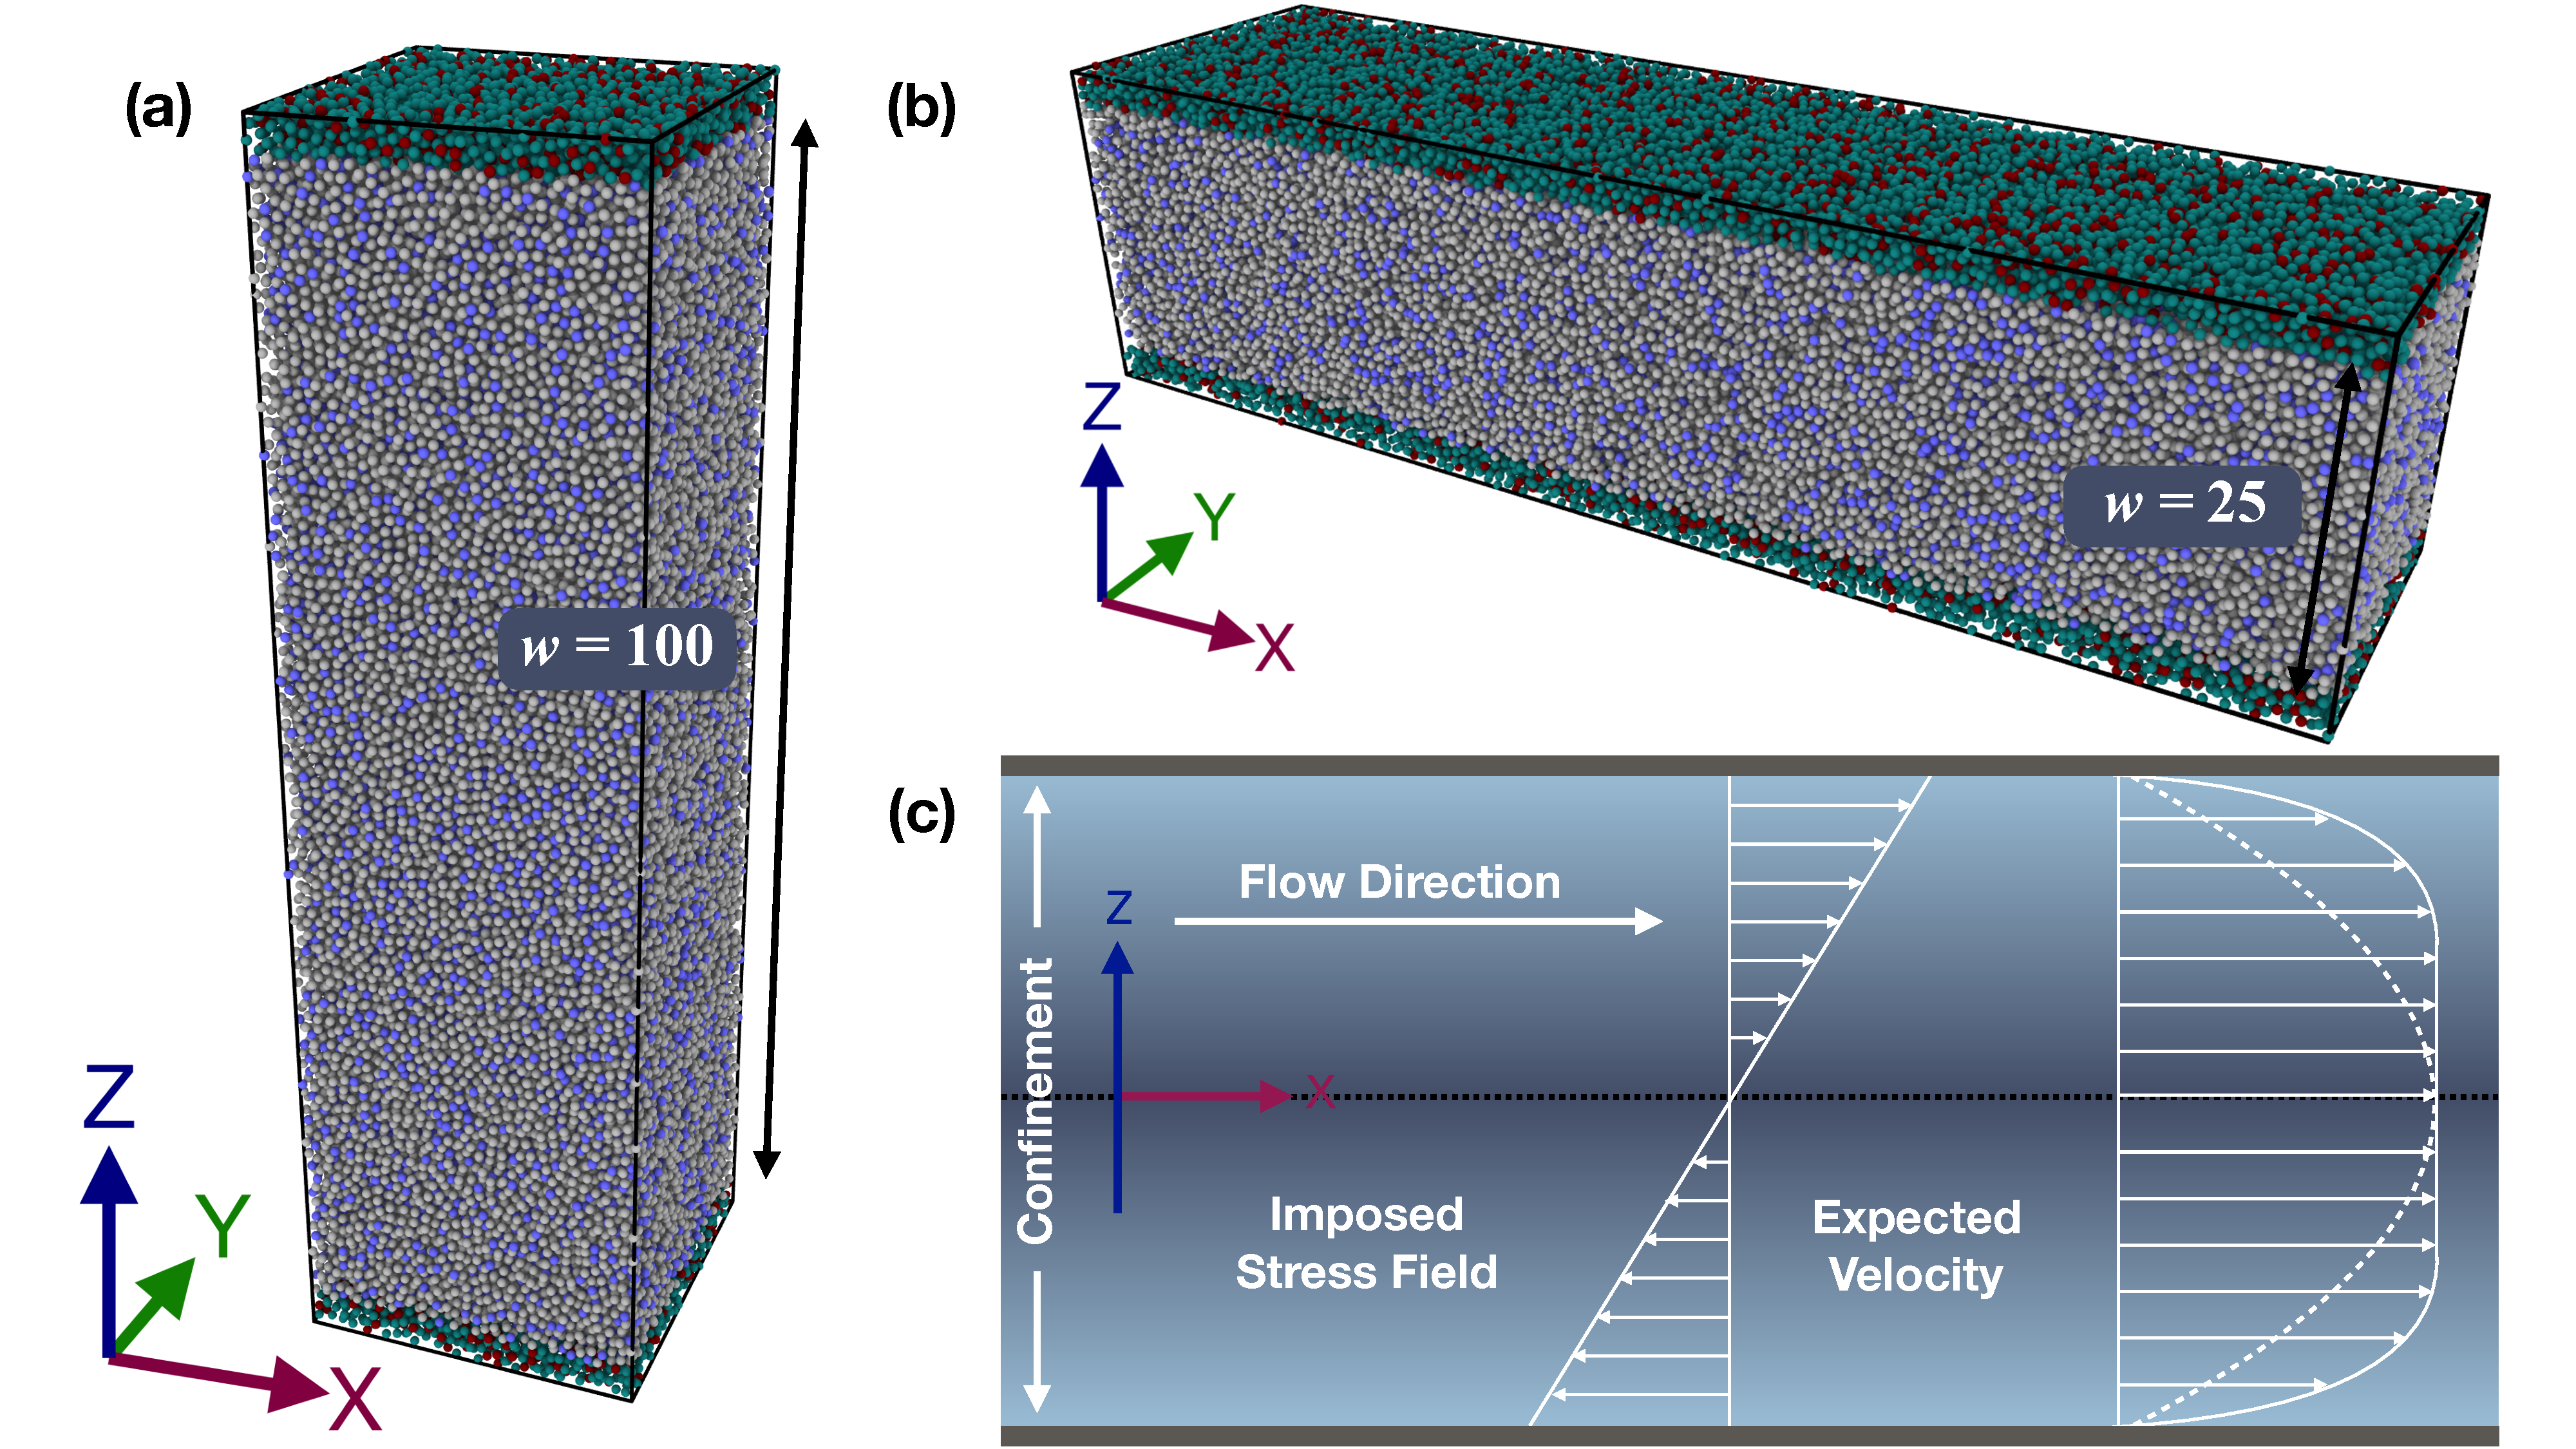
\includegraphics[width=15cm]{figs/schematicPoiseFlow.pdf}
\caption[{\em Schematic of Poiseuille flow geometry and snapshots of the binary LJ mixture confined between rough walls for two different channel widths}]{Schematic of flow geometry. Snapshots of the binary LJ mixture, confined between rough walls along the $z$ direction, is shown for (a) wide [$w=100$] and (b) narrow [$w=25$] channels. The external forcing which generates the Poiseuille flow is along the $+x$-direction, as marked in (c), and the shear thus develops in the $xz$ plane, with the resultant shear stress profile schematically illustrated in (c). Also shown schematically in (c) are the expected velocity profiles for a Newtonian and a yield stress fluid, which respectively correspond to parabolic or blunt profiles.}
\label{fig0}
\end{figure}
%%%%%%%

\subsection{Couette flow}

We also compare some results of the Poiseuille flow with those of the Couette flow, where the shear is imposed by fixing the shear-rate, corresponding to which a uniform shear stress is maintained. The Couette flow simulations are done for $N=8000$ particles in a cubic box with periodic boundary conditions in all three directions and the fixed shear-rate is imposed by deforming the box at the corresponding rate \cite{PhysRevE.102.023002} and simultaneously integrating the equations of motion of the particles. The required ambient temperature is maintained via a DPD thermostat (check section-\ref{thermostat} of Chapter-\ref{chap2} for more details about DPD thermostat) \cite{shrivastav2016yielding}.

\subsection{Implementation of thermostats}

The applied forcing to maintain Poisuille flow also leads to the generation of heat. If a thermostatting mechanism removes the excess heat generated, then a steady state is achieved where rate of heat generation becomes equal to the rate of heat removal. In this stage, a steady profile of different quantities like temperature, velocity of flowing particles, stress etc is maintained. Different thermostatting procedures have been adopted in various studies related to flow in confined channels \cite{hartkamp2017,luding2007,yethiraj1997}. In this study, we will consider two such thermalisation procedures and study how the flow of a glass forming material is influenced by the nature of the thermostat.

For the construction of the thermostats, we consider two kinds of confining walls: first is the \textit{vibrating wall}  and second is the \textit{frozen wall}: (i) In the case of vibrating wall, particles are tethered to their initial positions (at $t_{age} = 10^4$) and at each time-step, experiences a harmonic force equal to $-\kappa r$, where $\kappa$ is the spring constant and $r$ is the displacement of the particle with respect to initial position \cite{thompson1990,powles1992,todd1995,evansMorrissBook,koplik2001,varnik2002,koplik2006}. Such a wall consisting of vibrating particles does not allow the confining particles to escape. The wall particles keep interacting among each other and  with the confining fluid in the channel, resulting into continuous exchange of momentum and energy between wall and fluid particles. Further, each of the walls consists of three different layers (each of thickness unity) and the velocities of the particles in each layer is separately rescaled to the target temperature $T = 0.4$ at each time-step\cite{kim2008}. Fluid particles in the channel are not coupled to any separate thermostat, their dynamics is solely influenced by the two walls. This mechanism is able the maintain a constant temperature in the channel in the absence of any external forcing, as we will demonstrate below. Also, the dynamics of the fluid particles is not perturbed because of any coupling to external heat bath, making this probably the most natural way to remove the excess heat generated in the system, closely mimicking the experimental conditions. In the discussion below, we will refer to this thermostatting process as the "wall thermostat".
(ii) In the case of second type of wall, particles building the wall are frozen at their respective positions at $t_{age} = 10^4$  by setting their velocity to zero and fixing the forces acting to zero\cite{pinaki2014}. The temperature of the  fluid particles is maintained at a certain temperature via a DPD thermostat (using dissipation constant unity)\cite{dpd}, which does not introduce any bias in the spatial profiles of the emergent flow (check section-\ref{thermostat} of Chapter-\ref{chap2} for more details about DPD thermostat). Henceforth we will refer to this thermostat condition as the "DPD thermostat".


\section{Results}

\subsection{In the absence of shear}

We first compare the structural and thermal state inside the channel, in the absence of external forcing, for the two thermostatting methods.  The corresponding data is shown in Fig.\ref{fig1}.  As expected, in both cases, the temperature profile $T(z)$ is identical across the channel; see  Fig.\ref{fig1} left panel. However, there is a difference, as visible from the temperature profiles. For the wall thermostat, the wall temperature is maintained at $T=0.40$, whereas for the DPD thermostat, the wall temperature is zero since the particles constituting the wall are completely frozen. Next, for the two thermostat conditions, we examine the density profile $\rho(z)$ and observe that the structure is also the same across the channel; the local density fluctuates around the mean density of 1.2 as can be seen in  Fig.\ref{fig1} right panel.  Hence, in the absence of any external drive, the two thermostats provide similar thermal and structural conditions.
%%%%%%%
\begin{figure}
\centering
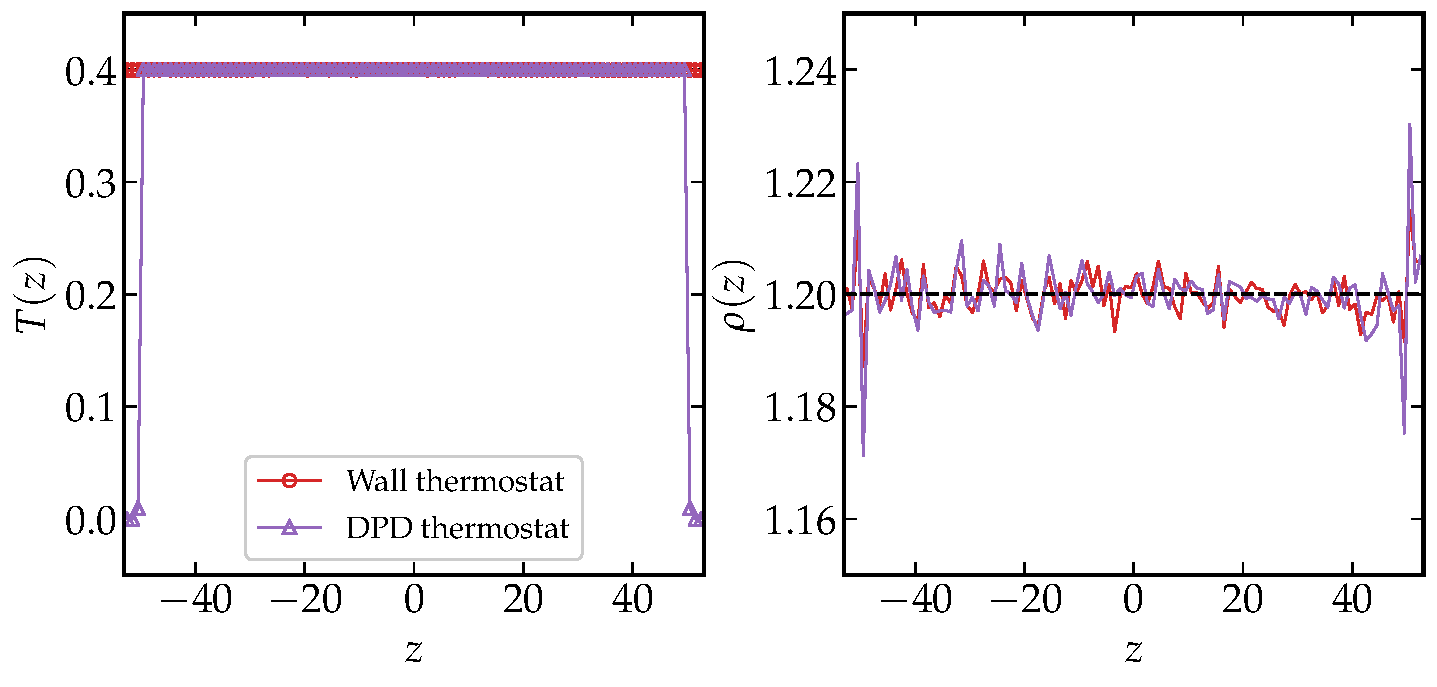
\includegraphics[width=15cm]{figs/compThermostat.pdf}
\caption[{\em Temperature and density profiles in the absence of flow}]{In the absence of flow, comparison of temperature $T(z)$ (left) and density profiles $\rho(z)$ (right), for the two thermostats as labelled.}
\label{fig1}
\end{figure}
%%%%%%%

Note that for computing these spatial profiles as well other profiles to be discussed later, we have subdivided the $z$-direction into layers of thickness $dz = 1$ parallel to $xy$-plane and averaged the data along $x$ and $y$ directions within each such layer, to obtain the spatial profiles that we report.


\subsection{In the presence of shear: steady state}

First, we address the important question of how do the temperature profiles look like inside the channel, in steady state Poiseuille flow, for different applied external forcing. This is shown in Fig.\ref{fig3}. For the case of DPD thermostat, there is no difference in $T(z)$ with increasing magnitude of forcing, within the range explored -- it is spatially uniform across the channel; see right panel of Fig.\ref{fig3}. On the other hand, for the case of wall thermostats, the temperature across the channel not only varies, with a maximum at the centre of the channel, but also this maximum value is dependent on the external forcing -- the larger the forcing, the larger is the local temperature; see left panel of Fig.\ref{fig3}. Due to this non-uniform thermal conditions, some  regions even have local temperature above $T_{MCT}$, i.e. those regions are in the supercooled state and therefore should impact the rheological behaviour of the system. Note that, in the case of both thermostats, for computing the temperature profiles accurately via the local kinetic energies, we subtract the local mean streaming velocity and thereby use the instantaneous velocity fluctuation in the flow direction \cite{todd1995}. For Newtonian fluids, the temperature profile is described by the following function \cite{todd1995, binder2004molecular}: $T(z)=T_0 + A(\rho_0{F_x}w^2)^2[1-(2z/w)^4]$, where $A$ is dependent on the thermal conductivity and the viscosity of the fluid (check section-\ref{PoiseuilleFlow} for the derivation of this expression for temperature profile). We check whether such a quartic function can fit the temperature profiles that we observe, which are shown in the left panel of Fig.\ref{fig3}, and note that the fits do not work. One of the reasons is that the fluid is not Newtonian, rather a yield stress fluid implying that the viscosity depends upon shear-rate and thus the above function does not provide a good description.

%%%%%%%
\begin{figure}
\centering
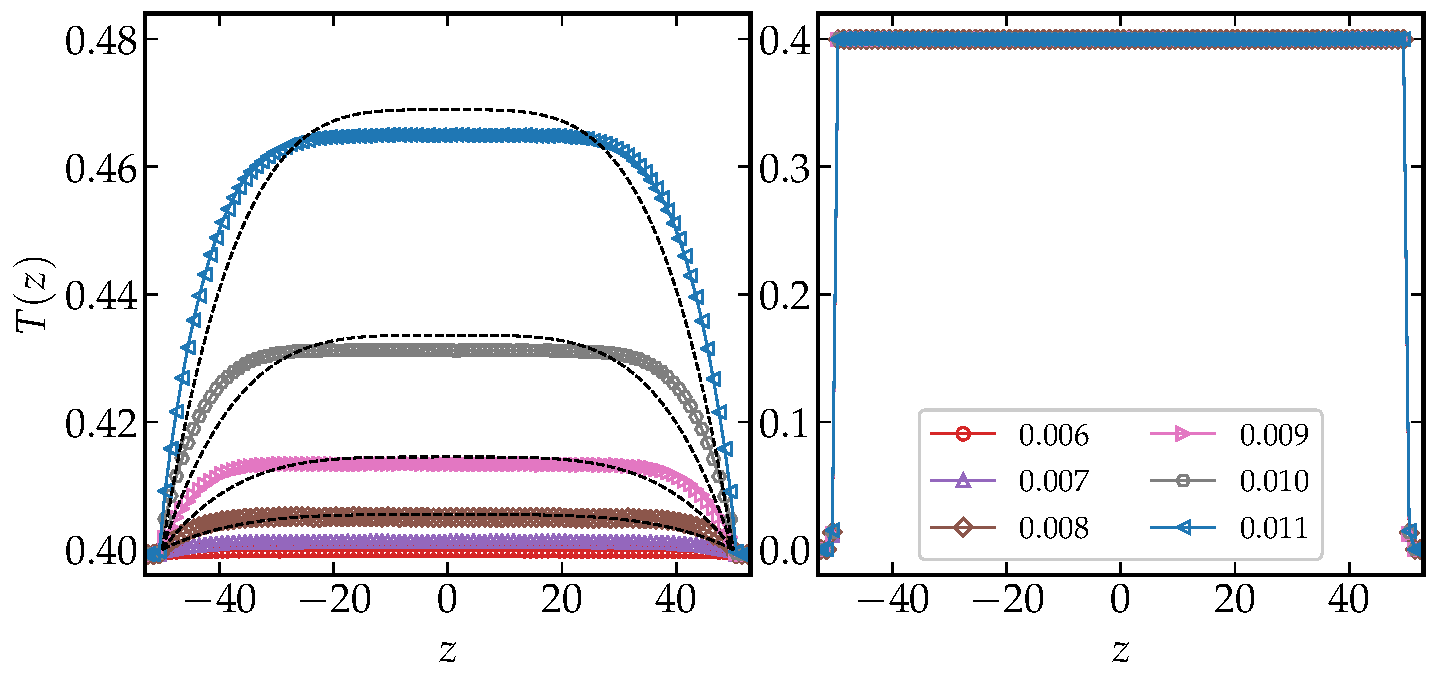
\includegraphics[width=15cm]{figs/tempComb.pdf}
\caption[{\em During Poiseuille flow, comparison of temperature profiles within the channel, in the presence of the two thermostats}]{During Poiseuille flow, comparison of temperature profiles within the channel, in the presence of the two thermostats, viz. wall thermostat (left) and DPD thermostat (right), for different strengths of the applied force (marked).  Also shown in the left panel, with dashed lines, are fits using the function $T(z)=T_0 + A(\rho_0{F_x}w^2)^2[1-(2z/w)^4]$, where A is a fit parameter.}
\label{fig3}
\end{figure}
%%%%%%%

%%%%%%%
\begin{figure}[htb!]
\centering
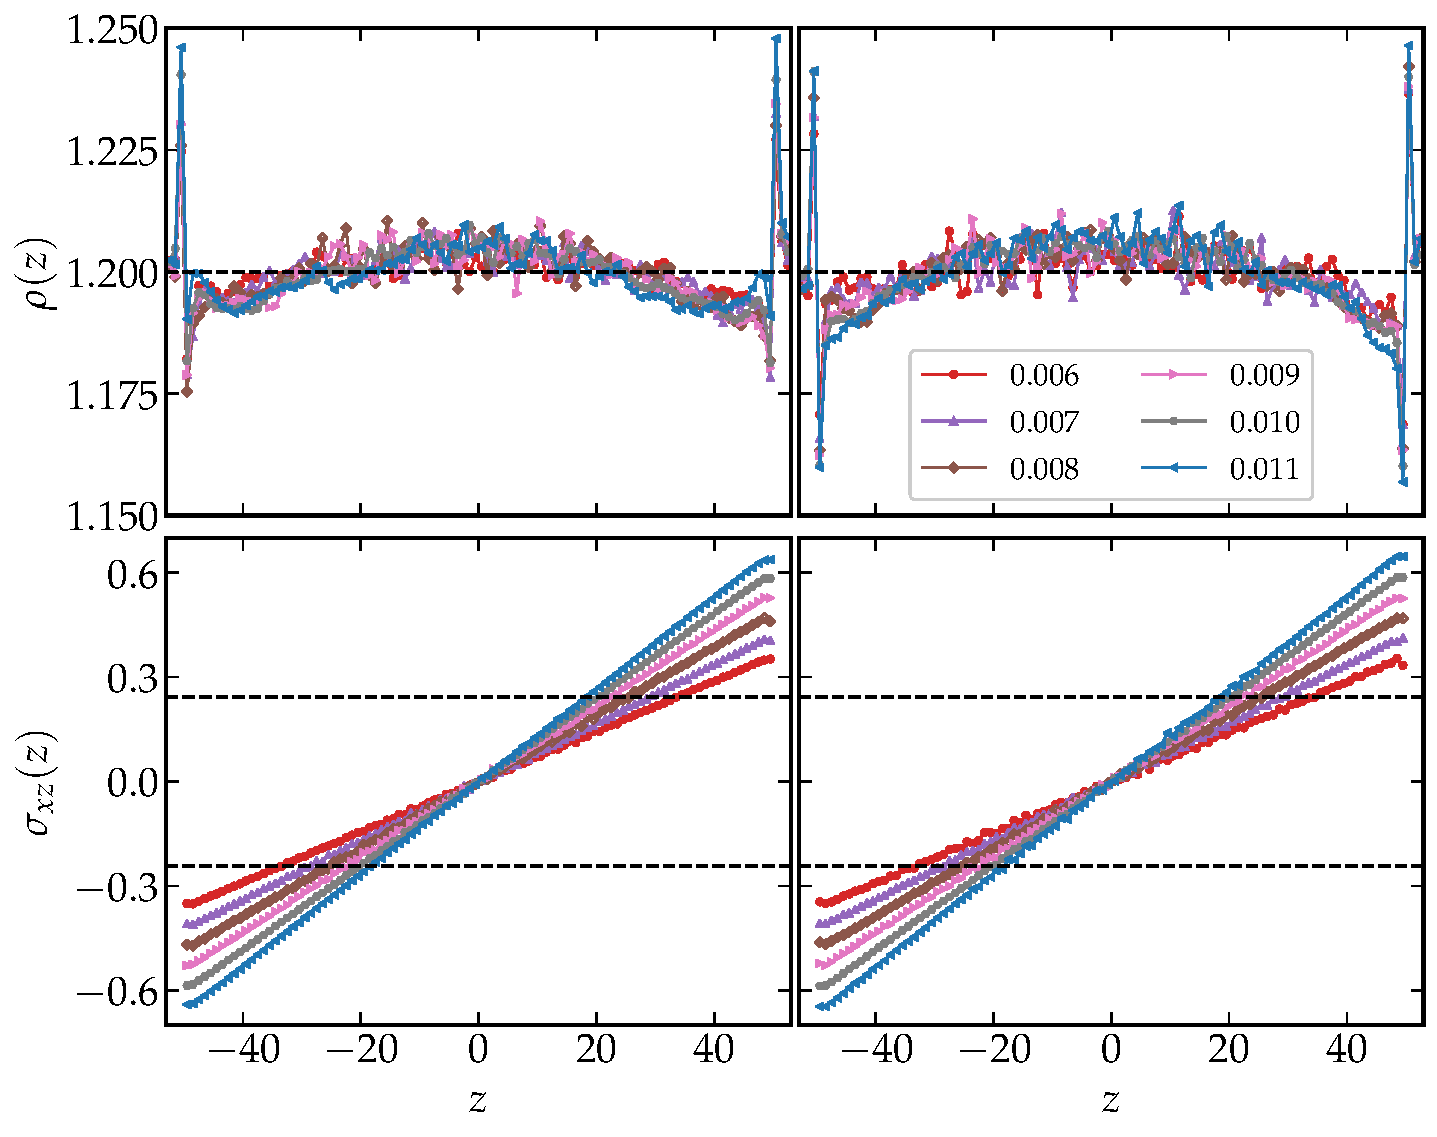
\includegraphics[width=15cm]{figs/denStress.pdf}
\caption[{\em Comparison of density and stress profiles in the presence of the two thermostats}]{Poiseuille flow. (Top) Comparison of  density profile, $\rho(z)$ in the presence of the two thermostats, viz. wall thermostat (left) and DPD thermostat (right), for different strengths of the applied force (marked). (Bottom) the shear stress profile emerging in the channel, for different strengths of the applied force (marked), in the presence of the two thermostats, viz. wall thermostat (left) and DPD thermostat (right). Also marked using dashed lines, in both left and right panels, is the bulk shear stress yield threshold ($\sigma_d=0.242$) at temperature $T=0.4$.}
\label{fig2}
\end{figure}
%%%%%%%

Having clarified the ambient thermal conditions, we analyse how the density profiles change when the external forcing is introduced in the form of Poiseuille flow. Here, we discuss the situation when the non-equilibrium steady state has been attained, for both thermostats, after application of the external force. The nearly flat density profile observed in the quiescent case is modified and there is some variation across the channel with a mild maximum at the centre of the channel; see Fig.\ref{fig2} top panel. The shape of the density profiles seems to be roughly similar for both the thermostats that we have studied. In general, such spatial variation hints at shear-induced migration effects, which we will discuss later.

We have then computed the shear-stress profiles building up inside the channel, as we vary the external forcing, using the standard Irving-Kirkwood expression \cite{todd1995pressure}. The corresponding data is shown in Fig.\ref{fig2} bottom panel. The shear stress profiles for both thermostats are identical and has the spatially linear profile, as is expected from mechanical stability \cite{todd1995pressure}. We also mark on the plots the bulk yield stress value ($\sigma_d \approx 0.24$) estimated from Couette flow measurements at the same temperature ($T=0.4$). We note that the naive expectation is that for each applied forcing, the spatial regions having local stress between $\{-\sigma_d, \sigma_d\}$ would see no flow, i.e. the local shear-rate should be zero. We analyse this aspect, further, below.

Hence, the different local thermal conditions for the two different thermostats do not affect the structural properties and thus the shear stress field that is set up. 


%%%%%%%
\begin{figure}
\centering
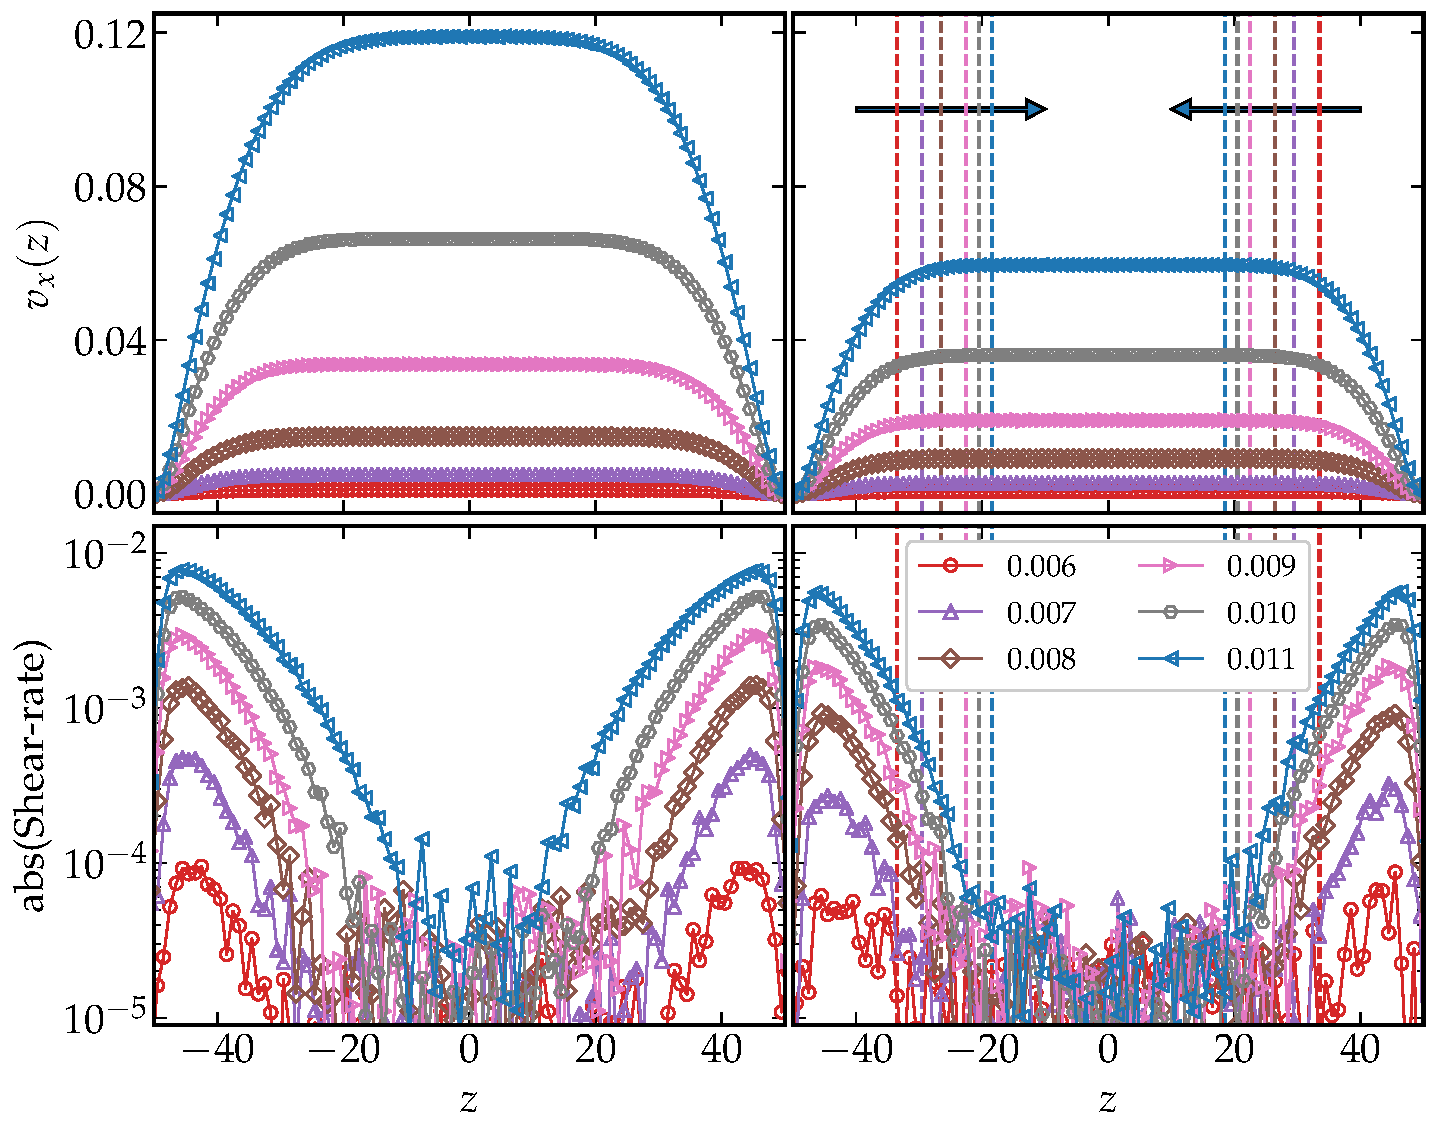
\includegraphics[width=15cm]{figs/velVelGrad.pdf}
\caption[{\em Steady state velocity profiles and corresponding spatial profile of local shear-rates for the different strengths of the applied force, for the two thermostats}]{Poiseuille flow. Steady state velocity profiles (top) and corresponding spatial profile of local shear-rates (bottom), for the different strengths of the applied force (marked), and for the two thermostats, viz. wall thermostat (left) and DPD thermostat (right) In the right panel, the zones within each pair of vertical dashed lines (having same color) correspond to the region where the local shear stress is below the bulk yield threshold at $T=0.40$ for each external forcing (same colored lines). The arrows in the top right panel indicate the direction of increasing $F_x$ for the sequence of vertical dashed lines.}
\label{velocityprofiles}
\end{figure}
%%%%%%%



Now, we address the important question whether the rheological response differs under these contrasting thermal conditions. The first check is via the velocity profiles observed in steady state, in the case of the two thermostats. As can be seen in the top panel of Fig.\ref{velocityprofiles}, the shape of the velocity profiles is consistent with what is observed for Poiseuille flow of soft glassy materials in wide channels. Unlike the parabolic flow of Newtonian fluids, here we observe blunted profiles due to the underlying Herschel-Bulkley shape of rheological curves, which we will further discuss below.  Consequently, the spatial profile of local shear-rates has a non-linear shape, compared to the linear shape expected for Newtonian fluids; see bottom panel of Fig.\ref{velocityprofiles}. At the centre of the channel, it should be noted that the local shear-rate is not zero as should be the case for yield-stress fluids, but seems to have a finite value \cite{mansard2013molecular}. However, the local shear-rate signal is very noisy at the centre of the channel and it is difficult to ascertain any differences with changing magnitude of the external forcing. Note that simple fluidity models \cite{goyon2008spatial, chaudhuri2012dynamical} predict finite shear-rates in regions where the local stress is less than the bulk yield stress, via non-local effects \cite{bocquet2009kinetic} due to the interplay of elasto-plastic correlations intrinsic to glassy systems and the imposed stress gradient via the Poisuielle flow; but, this effect becomes weaker with increasing width of the channel.

When we compare the response to the same external forcing (e.g. $F_x=0.010$), for the case of the two thermalisation protocols, we first note that in the centre of the channel, where the profiles are blunted, the velocity is larger in the case of the wall thermostat than the DPD thermostat. Further, the central blunt region is also more narrow for the case of the wall thermostat, the curvature also changes and consequently the local shear-rate is higher at any region away from the centre of the channel. These are consequences of the existence of local thermal gradient as well as higher local temperature in that region, for the case of temperature control via the walls. 

At any fixed forcing $F_x$, the deviation in local temperature $T(z) - T_0$ scales with $F_x^2$, as derived for Newtonian fluids. Thus, with increasing $F_x$, there are larger local temperatures which implies larger shear-rates compared to the case of spatially uniform temperatures, and hence larger deviations in local velocity.

Note that in all cases, no slip is observed in the velocity profiles due to the choice of rough boundaries. Further, note that the non-monotonicity in the local-shear profiles occur where the amorphous boundaries begin, i.e. where the flow velocity becomes negligibly small.

%%%%%%%
\begin{figure}
\centering
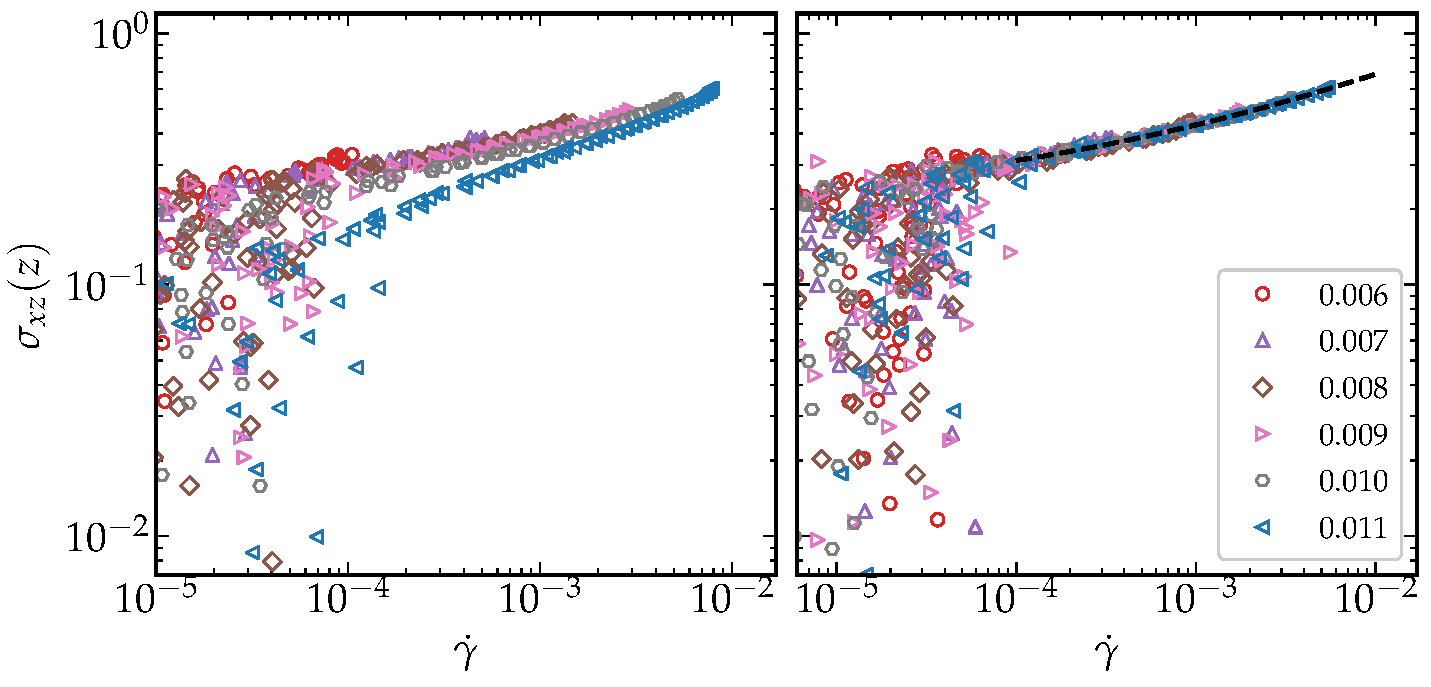
\includegraphics[width=15cm]{figs/stressStrain.pdf}
\caption[{\em Comparison of local flow curves for the different strengths of the applied force, corresponding to the two thermostats}]{Comparison of local flow curves, i.e. local stress vs local strain-rate, for the different strengths of the applied force (marked), corresponding to the two thermostats, viz. wall thermostat (left) and DPD thermostat (right). Also shown in the right panel, using a dotted line, is a Herschel-Bulkley fit to the collapsed data using $\sigma = \sigma_0 + K\dot{\gamma}^n$ with $\sigma_0 = 0.205$, $K = 2.188$ and $n = 0.328$.}
\label{localflow}
\end{figure}
%%%%%%%

%%%%%%%
\begin{figure}
\centering
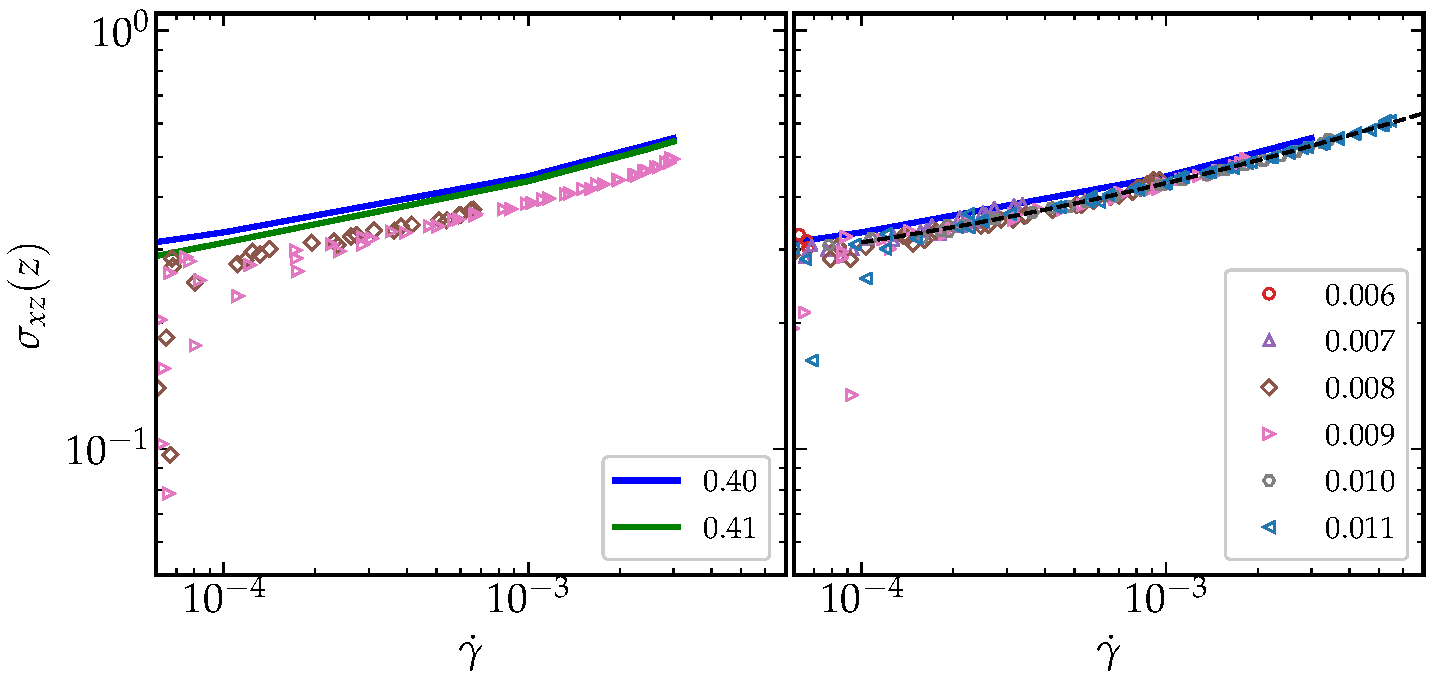
\includegraphics[width=15cm]{figs/stressStrain_0p41.pdf}
\caption[{\em Comparison with bulk rheology data obtained from Couette flow}]{Comparison with bulk rheology data obtained from Couette flow. (Left) Variation of stress with shear-rate during Couette flow at $T=0.40, 0.41$ (in lines, as marked), shown along with local stress vs local shear-rate data (in symbols) where local temperature is in the range $[0.405,0.415]$ obtained from Poiseuille flow with wall thermostat. (Right) Variation of stress with shear-rate during Couette flow at $T=0.40$, shown along with the aggregated data for Poiseuille flow using DPD thermostat and the corresponding Herschel-Bulkley fit [see Fig.\ref{localflow}].}
\label{couettecompare}
\end{figure}
%%%%%%%

Next, to analyse the rheological response in greater detail, we probe the dependence of local shear-rate on local stress. For each applied $F_x$, we know the spatial dependence of shear stress (see bottom panel of Fig.\ref{fig2}) and also the spatial dependence of the shear-rate (see bottom panel of Fig.\ref{velocityprofiles}). Hence, at each spatial location, we have information on how local shear-rate depends upon local shear stress. This, we can aggregate for the different magnitudes of external forcing, and then plot local shear-rate vs local stress, which is shown in Fig.\ref{localflow} for the two thermostats. For the case of DPD thermostat, the data for different imposed $F_x$ values collapse into a single master curve; there is some scatter at small local shear-rates which is due to the noisiness of the data at the centre of the channel. This collapsed data can be fitted by the Herschel-Bulkley form $\sigma = \sigma_0 + K\dot{\gamma}^n$ with $\sigma_0 = 0.205$, $K = 2.188$ and $n = 0.328$ as the fit parameters. On the other hand, for the wall thermostat, no such data collapse occurs; rather, there seems to be distinct branches for each $F_x$.

Further, we can verify how these local flow curves constructed from the Poiseuille flow data for the local stress vs local shear-rates compare with the bulk rheology data obtained from Couette flow studies using periodic boundary conditions. Note that the shear stress is spatially homogeneous for the Couette flow, while it is inhomogeneous for the Poiseuille flow.The Couette flow simulations are done for imposed constant shear-rate. This imposed shear develops shear stress within the system, and the variation of the macroscopic shear-stress with the imposed shear-rate, constitutes the bulk rheological flow curve \cite{bonn2017yield}. This is in contrast to the local shear stress vs local shear-rate measurements that we are doing for the Poiseuille flow. The naive expectation is that for a wide enough channel, the local flow curve measured for Poisuielle flow would converge to the bulk flow curve, since it would ideally be a unique material property of the model system independent of rheological protocol. However, as has been demonstrated before \cite{goyon2008spatial, chaudhuri2012dynamical} , deviations are observed for a narrow channel, due to enhanced non-local effects occurring via the interplay between the inhomogeneous stress field and the intrinsic plastic correlations within a glassy system \cite{bocquet2009kinetic}.

First, we make the comparison between the bulk and local flow curves for the case of the DPD thermostat, where the temperature across the channel is maintained at the target temperature of 0.40; see right panel of Fig.\ref{localflow}. If we compare with the flow curve obtained from Couette flow, we see that there is some deviation, which is known to occur due to the non-local effects in channel flow as discussed above; even for channels as wide as 100 diameters, such effects cannot be ruled out. For the case of the wall thermostat, doing this comparison is non-trivial since the local temperature is also varying [see left panel of Fig.\ref{fig1}]. So, to do a first comparison between local and bulk flow data for this situation, we select one specific temperature value, viz. $T=0.41$. To obtain the data from Poiseuille flow, where there is a scatter of local temperatures around $T=0.41$, we consider cases where the the  local temperature is in the range of $[0.405,0.415]$ and for those zones, we collect the data for local stress and local shear-rate.  This is then compared with the Couette flow data computed for temperature $T=0.41$; see left panel of Fig.\ref{localflow}. We observe a large deviation -- at any particular local stress, the flowing glass has a larger shear-rate. Hence, it is evident that just by knowing the local temperature, it is not possible to predict the flow behaviour. Rather, there is enhanced plasticity as captured via the increase in local shear-rates, which would imply that the existence of both a stress gradient and temperature gradient significantly affects the rheology.

%%%%%%%
\begin{figure}[t]
\centering
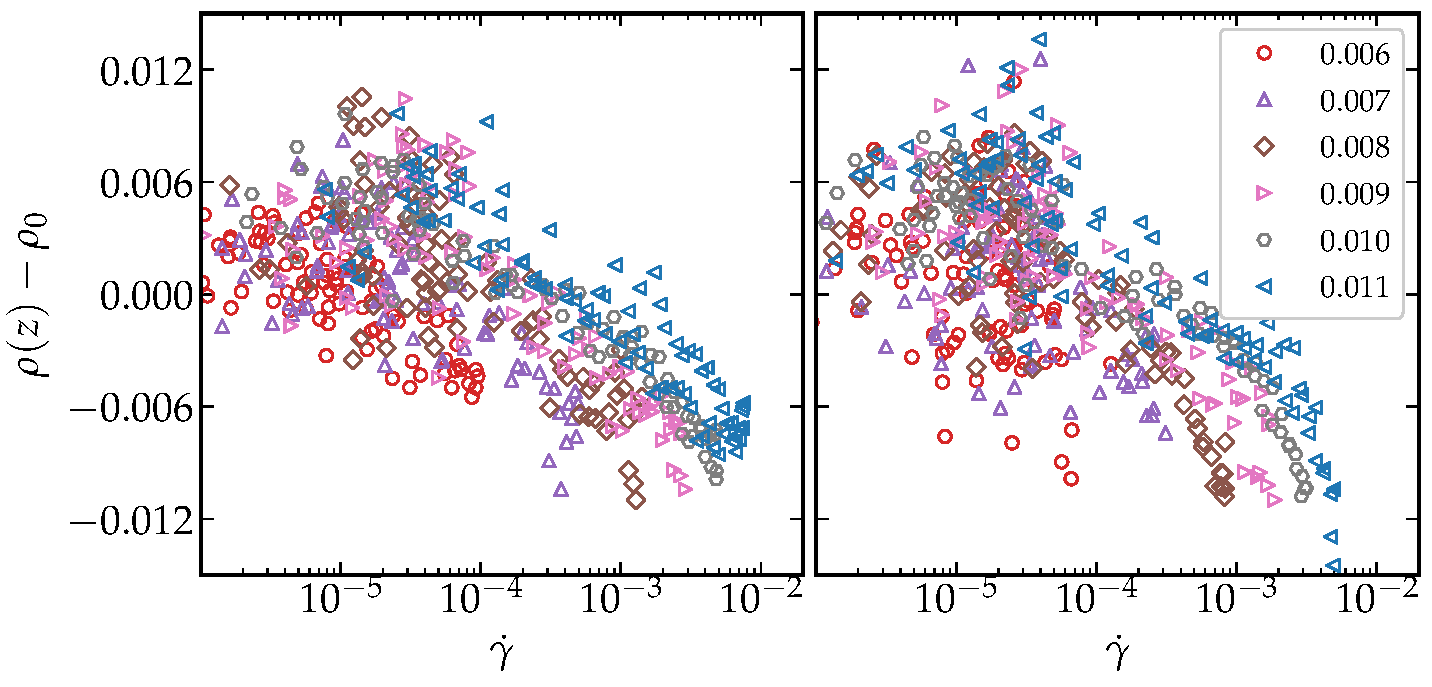
\includegraphics[width=15cm]{figs/denShrRt.pdf}
\caption[{\em Steady state variation in local density fluctuations with local shear-rate for wall thermostat and DPD thermostat}]{Steady state variation in local density fluctuations, $\rho_z-\rho_0$, with local shear-rate in the case of wall thermostat (left) DPD thermostat (right), characterising particle migration occurring due to shear.}
\label{migration}
\end{figure}
%%%%%%%

We observe that there is increasing decrease in local density with increasing local shear-rate and also an enrichment at lower shear-rates, which are consistent with previous observations. All these effects are more pronounced with increasing $F_x$. However, we note that the deviations are around $1\%$ for the largest forcing that we have studied. Further the effect seems slightly weaker in the presence of thermal gradients, i.e. for the wall thermostat. The presence of thermal current from the wall towards the centre, due to the thermal gradient, could be a counterbalancing factor, which needs further probing.



\subsection{In the presence of shear: transient behaviour}

%%%%%%%
\begin{figure*}
\centering
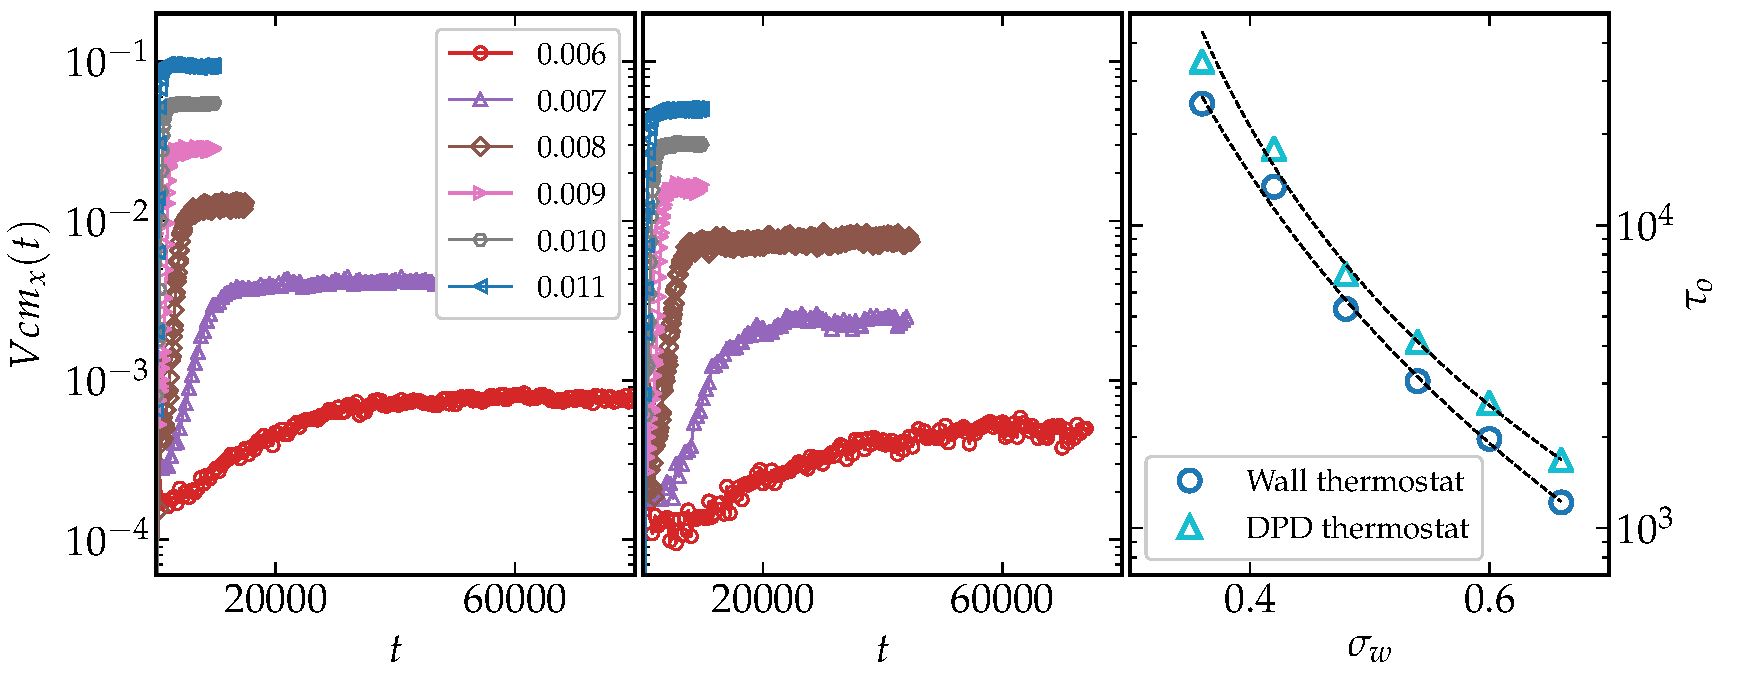
\includegraphics[width=15cm]{figs/vcmx.pdf}
\caption[{\em Transient Poiseuille flow: time evolution of mean flow velocity}]{Transient Poiseuille flow. Time evolution of mean flow velocity $v_{cm_x}$ from quiescence to steady-state for different applied $F_x$ as marked, for wall thermostat (left) and DPD thermostat (middle). (Right) Variation of the corresponding  timescale for onset of steady state $\tau_0$ for different magnitudes for external drive characterised by the wall stress $\sigma_w=\rho{F_x}w/2$, for the two thermalisation conditions.}
\label{onset}
\end{figure*}
%%%%%%%

%%%%%%%
\begin{figure}
\centering
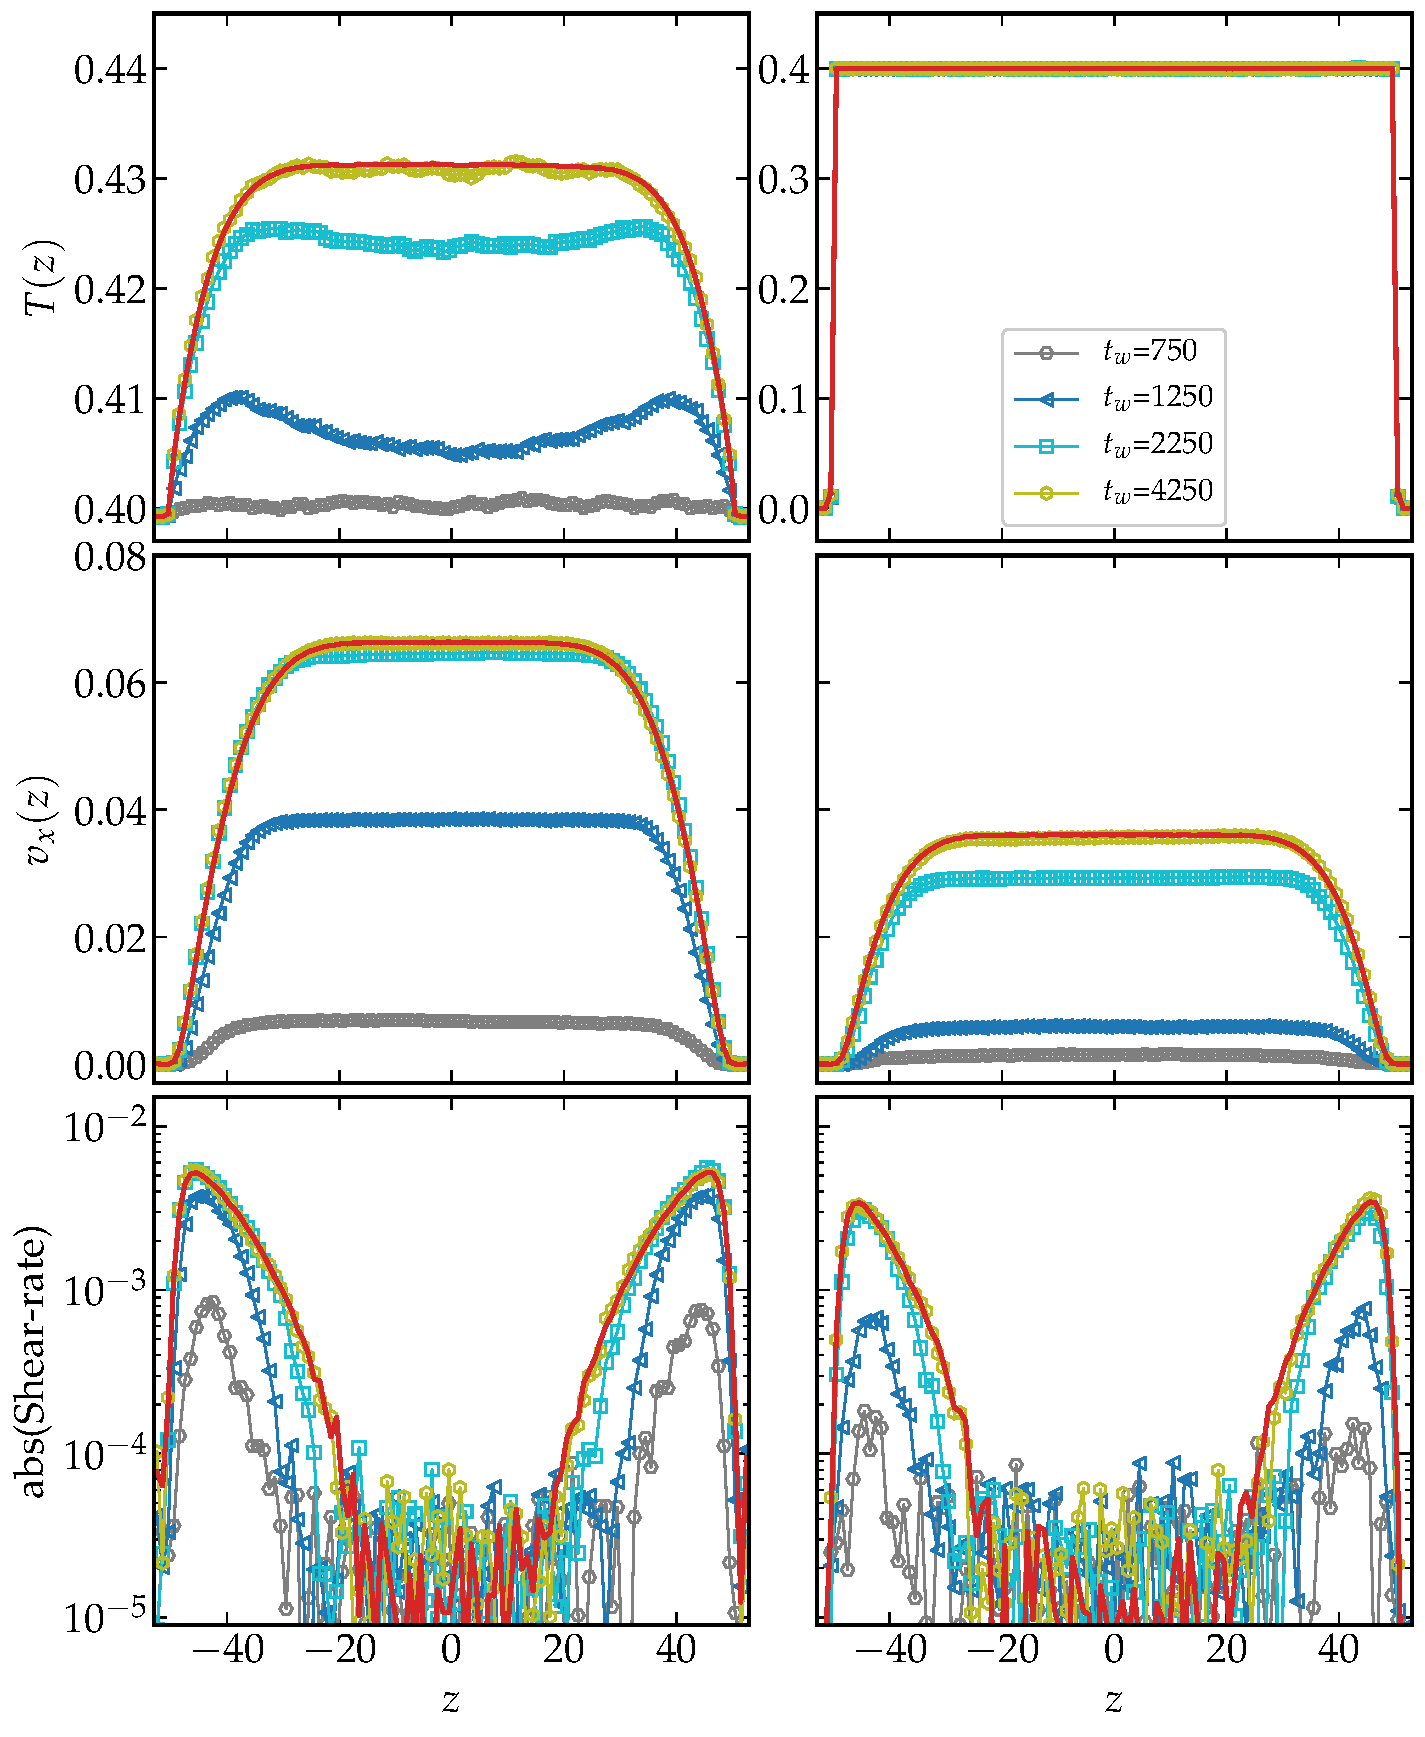
\includegraphics[width=15cm]{figs/profDev.pdf}
\caption[{\em Transient Poiseuille flow: development of spatial profiles of temperature, velocity and shear-rate, for the wall thermostat and DPD thermostat}]{Transient Poiseuille flow. Development of spatial profiles of temperature (top), velocity (middle) and shear rate (bottom), with time (as indicated) after imposition of a forcing $F_x = 0.010$; left panel corresponds to the wall thermostat and the right panel corresponds to the DPD thermostat. For each observation time, data has been averaged over a period of $\delta t = 250$ around the indicated time. Solid line is the steady state behaviour that is eventually observed.
}
\label{onset2}
\end{figure}
%%%%%%%


Having analysed the steady state flow behaviour, we now investigate the way to steady state from the initial quiescence, after the imposition of the external forcing. This can be studied by monitoring the mean flow velocity in the direction of flow \cite{pinaki2014}, $v_{cm_x}$, for the different applied $F_x$, and this is shown in the left and middle panels of Fig.\ref{onset} for the wall thermostat and DPD thermostat conditions, respectively. In the absence of the external drive, the average flow velocity is of course zero. When the external drive is switched on, $v_{cm_x}$ increases over a certain time window and eventually settles to a finite steady value, which increased with increased forcing. Further, as discussed above, we note that the steady state value of $v_{cm_x}$ is larger under wall thermostat conditions, for a fixed magnitude of the external forcing, implying that the flow is faster. We can study this further by focusing on the time evolution of the spatial profiles of velocity and temperature, for the same fixed force, but different thermostats, which we illustrate in Fig.\ref{onset2}. In the top panel, we show the time evolution of the temperature profile $T(z)$. For the DPD thermostat, the local temperature is always at the set value of 0.4. On the other hand, for the wall thermostat, $T(z)$ induced by the external force, emerges with time, before reaching the steady state profile.  Next, if we focus on the velocity profiles, shown in the bottom panel of  Fig.\ref{onset2}, we see that these also gradually evolve with time, for both thermostats, as expected. However, as can be easily seen, this is faster for the wall thermostat and the changes are happening as the local temperature also evolves towards steady state. Hence, the emergence of flow and thermal conditions are interlinked in this case.

Next, for each value of $F_x$ and for both the thermostat conditions. we estimate the timescale for the onset of steady state, $\tau_0$, by measuring when $v_{cm_x}(t)$ reaches the terminal steady state value. In the right panel of Fig.\ref{onset}, we show the variation of $\tau_0$ with each forcing characterised by the wall stress $\sigma_w=\rho{F_x}w/2$. First, we note that as expected \cite{pinaki2014}, the timescale for the onset of steady flow increases with decreasing $\sigma_w$. Further, we also note that for any particular $\sigma_w$, $\tau_0$ is larger in the presence of the DPD thermostat than the wall thermostat; the faster flow leads to faster onset of steady state. One can also then expect that the threshold in  $\sigma_w$, i.e. where $\tau_0$ is predicted to diverge, decreases for the case of the wall thermostat due to the presence of the thermal gradient.



%%%%%%
\begin{figure}
\centering
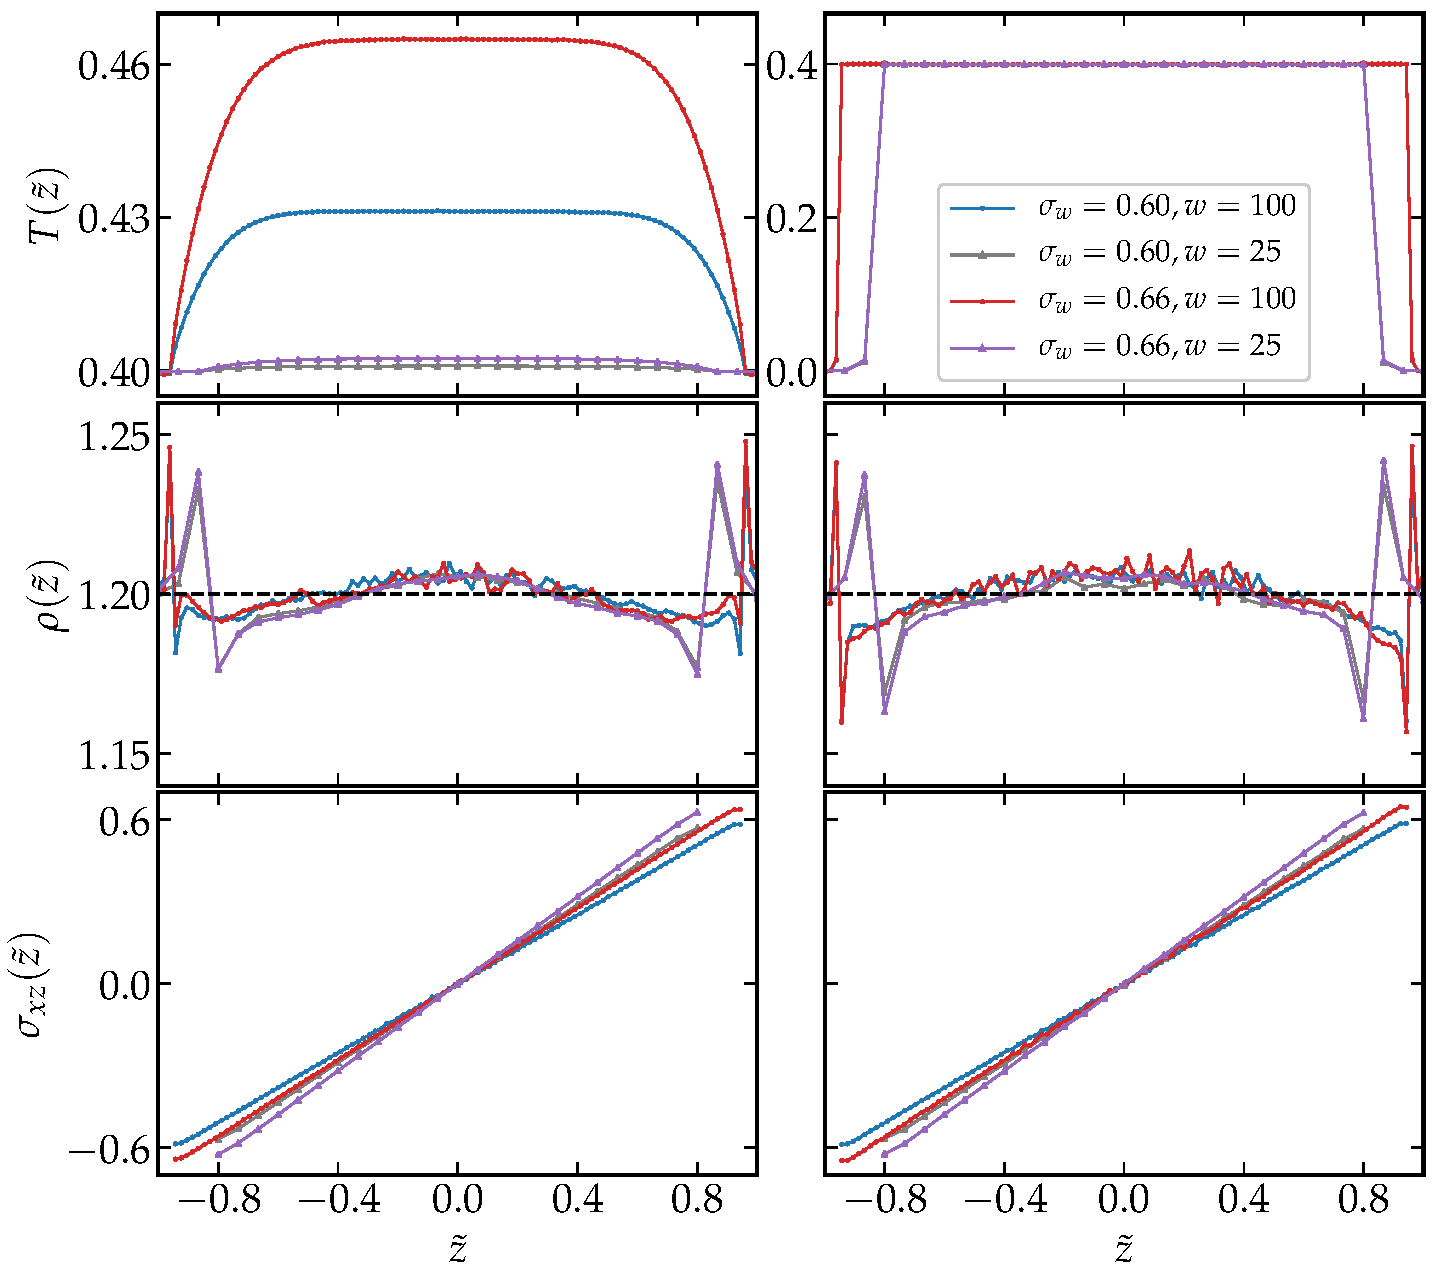
\includegraphics[width=15cm]{figs/cw1.pdf}
\caption[{\em Comparison of response for wide $w=100$ and narrow $w=25$ channels: spatial profiles of temperature, density, shear stress}]{Comparison of response for wide $w=100$ and narrow $w=25$ channels. Spatial profiles of temperature (top), density (middle), shear stress (bottom). In each case, left panel is data
for wall thermostat and right panel is for DPD thermostat. Note that $\tilde{z}$ corresponds to the scaled distance $\tilde{z}=2z/w$.}
\label{narrow1}
\end{figure}
%%%%%%%

\subsection{In the presence of shear: changing channel width}

We have also done some studies for a narrower channel ($w=25$), and we compare the observations with that for $w=100$ for a couple of wall stress values, viz. $\sigma_w=0.60, 0.66$, which provides the correct scale for comparing across different channel widths \cite{mansard2013molecular}.

First, if we compare the obtained temperature profiles in the case of wall thermostat, as shown in the top panel of Fig.\ref{narrow1}, the maximum temperatures observed are much less in the narrower channel. We recall that $T(z) - T_0 \propto \sigma_w^2w^2$, implying that narrower channels will witness lower temperatures for the same $\sigma_w$ even though the non-uniformity is still there. 

The density profiles, shown in the middle panel of Fig.\ref{narrow1}, exhibit oscillations due to layering effects for the narrow channel and this oscillations seems more pronounced for the DPD thermostat since the wall particles are static in that case. The shear stress profiles, shown in the bottom panel of  Fig.\ref{narrow1}, reveal deviations from the expected linear spatial profiles, which is related to the density oscillations with increasing confinement.


%%%%%%%
\begin{figure}
\centering
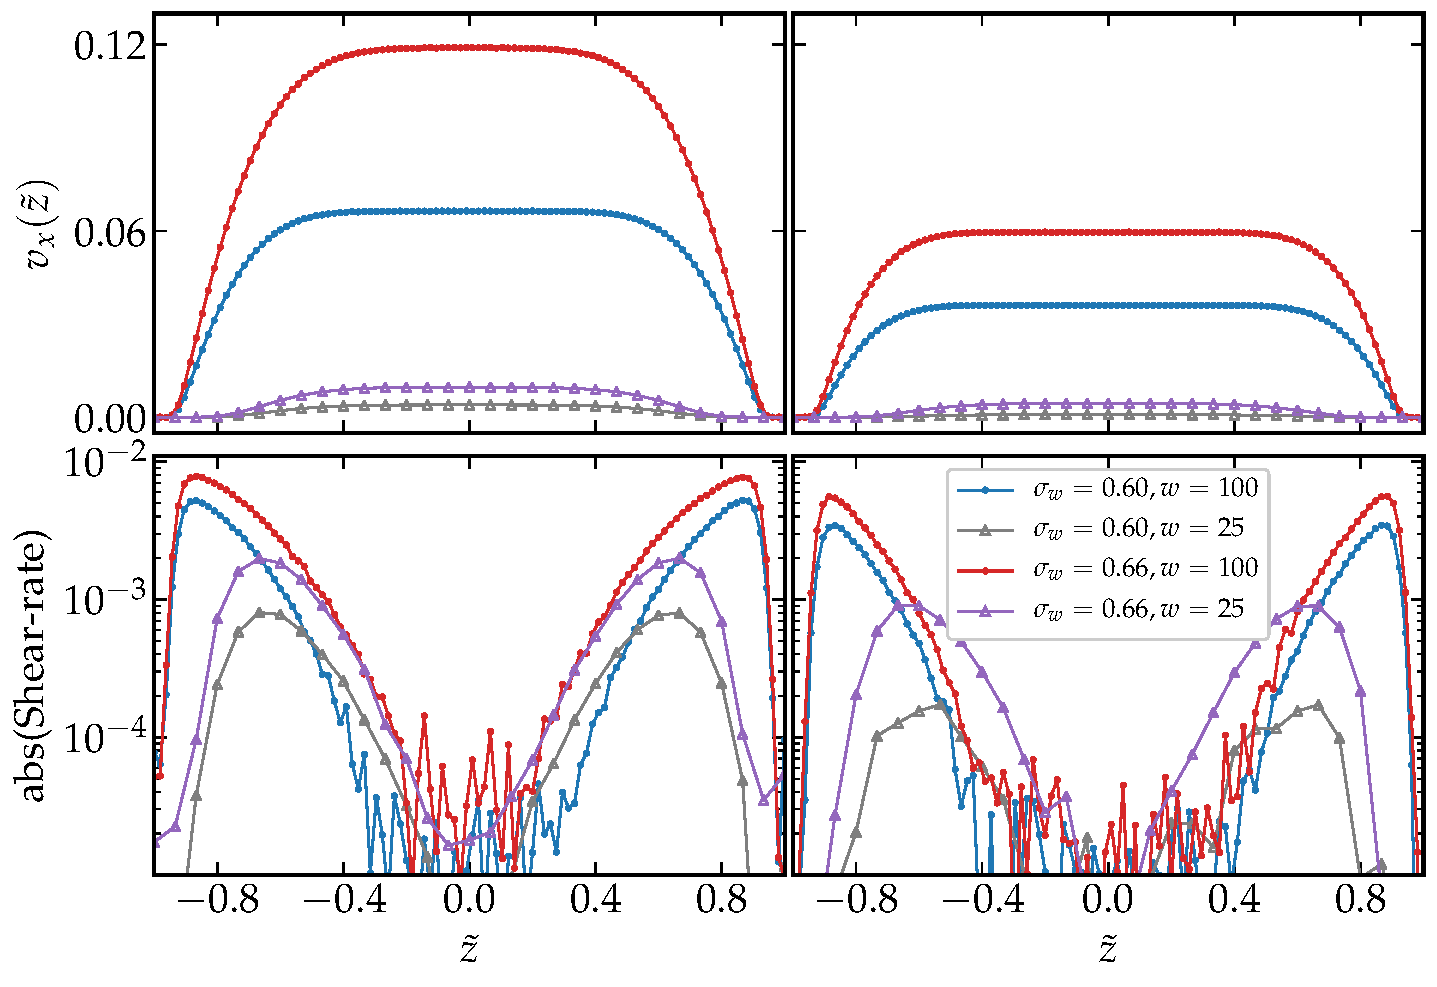
\includegraphics[width=15cm]{figs/cw2.pdf}
\caption[{\em Comparison of response for wide $w=100$ and narrow $w=25$ channels: spatial profiles of velocity and shear rate}]{Comparison of response for wide $w=100$ and narrow $w=25$ channels. Spatial profiles of  velocity (top), shear-rate (bottom). In each case, left panel is data
for wall thermostat and right panel is for DPD thermostat. Note that $\tilde{z}$ corresponds to the scaled distance $\tilde{z}=2z/w$.}
\label{narrow2}
\end{figure}
%%%%%%%

Next, we focus on the flow properties, viz. the local shear-rate profiles that are set up as shown in the bottom panel of Fig.\ref{narrow2}. In the case of DPD thermostat, decreasing channel width leads to increased curvature of the velocity profiles at the centre of the channel and thus increased local shear-rates, as observed in the right panel of Fig.\ref{narrow2}. This is a known consequence of the enhanced non-local effects with increasing confinement \cite{goyon2008spatial, mansard2013molecular}. 

However, for the case of the wall thermostat, the effect seems more complicated, due to the additional interplay with the non-uniform thermal conditions. For the smaller $\sigma_w$, if we compare the responses within the wide and the narrow channel,  the local shear-rates do get enhanced for the narrower channel; see left bottom panel of Fig.\ref{narrow2}. However, this is not the case for the higher $\sigma_w$, where the local shear-rates at the central region of both the wide and narrow channels seems comparable. One can understand this in the following way. There are two competing sources for enhancing local plasticity, one the increasing stress gradient and the other the thermal gradient. In the case of the wide channel, the thermal gradient is larger, whereas for the narrower channel, the stress gradient is larger. It seems that these competing effects get compensated leading to comparable rheological response in the central region for the two channel widths.  However, we also note that if we compare the response in the narrow channel for the DPD and the wall thermostat, the local shear-rates are higher in the latter case, implying that the thermal gradient, however small, does play its role in enhancing local plasticity.

Thus, this analysis gives us a glimpse into the complex interplay between the different existing gradients, viz. thermal and shear stress, and the correlated plastic processes intrinsic to glassy systems, which need further investigation.

\section{Conclusions}

In this work, we have studied the Poiseuille flow of a model soft glass, using two different thermalisation protocols. In one case, the confined material is thermalised via the walls, which are kept at the target temperature. Such a thermostatting procedure seems close to several practical applications where temperature control is easier to maintain via the confining walls, e.g. a complex fluid confined between hot or cold walls. In the other case, we thermalise the fluid directly and the particles constituting the walls remain completely frozen. Such a thermalisation procedure is also possible in diverse applications. The temperature targeted for thermalising is below the mode coupling temperature, but above the glass transition temperature, and thus in the ageing regime. In both cases, the walls are amorphous in nature, with the structure matching that of the confined aged glass. We emphasise that our objective is to study the rheological response of the confined glass under these different thermal conditions, and not a comparison of the efficacy of thermalisation via the two different thermostats under flow conditions.

In the absence of any external drive, uniform thermal profiles occur across the channel for both thermostat conditions. However, in the case of wall controlled thermalization, when Poiseuille flow is set up, there is a non-uniform temperature profile  existing across the channel in the shear gradient plane, similar to previous studies of other confined fluids. Of course, this is in contrast to the case where the fluid is directly thermalised; there, the temperature remains spatially uniform even in the presence of the flow. Thus, the process of thermalisation via the walls provides an opportunity to study the rheological response of the glassy system under the non-uniform thermal conditions, and to probe how this additional perturbation influences flow behaviour in conjunction with the imposed stress gradient due to the Poiseuille setup.

We observe that the structural properties, viz. the density profile and the shear-stress profile, do not vary under the different thermal conditions of the two thermostat protocols. However, there is a distinct difference in the observed flow behaviour. The mean flow is faster in the case of the wall-controlled thermostat, due to the increased local temperatures in the centre of the channel, and the difference with the fluid-controlled thermostat increases with increasing forcing, since the maximum local temperature that is set up scales with the magnitude of the external drive. This leads to larger local shear-rates across the channel width for the same scale of forcing, due to the non-local coupling between the spatially varying stress, thermal gradient and the spatial plastic correlations that are characteristic to glassy systems. As a consequence, the onset of flow also happens at a quicker timescale for the wall-controlled thermostat and we estimate that the stress threshold for yielding in the case may also be lowered, which can be utilised in practical applications. When we construct local flow curves in steady state, the data for different magnitudes of the external drives collapse in the case of the fluid-controlled thermostat, which can be fitted to a Herschel-Bulkley function. This still deviates slightly from the bulk rheological flow curve at that temperature measured from Couette flow, which is  expected from the non-local effects characteristic to Poiseuille flow. On the other hand, for the wall-controlled thermostat, there is no collapse in the data for local stress vs local shear-rate, and even data for any chosen local temperature deviates quite a lot from the bulk Couette flow curve computed for that particular  temperature. Hence, there is a complex interplay between the thermal gradient that is set up via the flow and the elastoplastic correlations intrinsic to glassy systems. In the end, we provide a further glimpse of this interplay by probing how the rheology varies if we decrease the channel width, where more complexities in response are observed via the competing effects of the presence of stress and thermal gradients, which need to be disentangled in future studies.

%This also needs to be studied via simple phenomenological formulations like the fluidity models \cite{mansard2013molecular} to examine the interplay of stress and temperaature gradients and corresponding correlations, to thereby evaluate rheological responses under diverse conditions, which can then be tested via numerical simulations. A starting point for theoretical formulations to understand these aspects could be the recent study on building constitutive equations for the case of shear inhomogeneities resulting from under-damped dissipation during external shear of amorphous materials \cite{vasisht2018permanent}. Beyond this, other nonequilibrium consequences
%\cite{vaibhav2020response} of a thermal gradient on glass-forming mixtures and its effects on local rheology needs to be investigated in details. 

Overall, we hope our study in this chapter, will motivate further exploration of how dissipation processes can influence the rheological response of confined soft glasses, both using experiments and theoretical or numerical initiatives, specially in the context of different shear protocols where diverse gradients emerge, and how these can be harnessed for useful applications, be it in industries or even in control of natural processes. 

